\section{The Axio-Dilaton Sector and 12d Gravity}
\label{sec:axio-dilaton-12d}
We now turn to the 12d structures suggested by brane solutions.
This higher-dimensional effective description is in parallel with what is known between the type IIA theory and M-theory (Table~\ref{tab:iia-iib-uplift}).
The 12d interpretations of the type IIB D7 and D(-1) backgrounds were first identified in \cite{Vafa:1996xn,Tseytlin:1996ne}. Here we derive them explicitly, alongside the corresponding type IIA constructions, and use them to read off how the type IIB \SLZ{} duality acts geometrically in 12d.

\begin{table}[ht]
\centering
\begin{tabular}{lcc}
\toprule
 & \multicolumn{2}{c}{reduced on a circle or torus to}\\
\cmidrule(l){2-3}
higher-dimensional solution & type IIA (from 11d) & type IIB (from 12d)\\
\midrule
Kaluza-Klein monopole & D6 brane & D7 brane\\
pp-wave               & D0 brane & D($-1$) instanton\\
\bottomrule
\end{tabular}
\caption{The parallel that organises this chapter. 
Two solutions of eleven-dimensional supergravity reduce on the M-theory circle to the type IIA D6 brane and D0 brane. 
The same two geometries in twelve dimensions reduce on a torus to the type IIB D7 brane and D($-1$) instanton.}
\label{tab:iia-iib-uplift}
\end{table}
One can truncate the type IIB action \eqref{eq:sl2r_invariant_einstein_frame_action} to the axio-dilaton sector
\begin{equation}
2\kappa^2S=
\int d^{10}x\sqrt{-g}\left[
R-\frac{1}{2}\frac{|\partial \tau|^2}{\tau_2^2}
\right].
\label{IIB axio-dilaton action}
\end{equation}
For supersymmetric solutions, we solve for Killing spinors.
In the type IIB theory, the R-symmetry is local $SO(2)\cong U(1)$, and the Killing spinor equations are \cite{Bergshoeff:2006jj}
\begin{equation}
\begin{aligned}
\delta\lambda
&=\frac{i}{\tau-\bar\tau}(\Gamma^\mu\partial_\mu \bar\tau)\epsilon,\\
\delta\psi_\mu
&=
\left(
\partial_\mu+\frac{1}{4}w_\mu{}^{ab}\Gamma_{ab} -\frac{i}{2}\frac{\partial_\mu \tau_1}{2\tau_2}
\right)\epsilon
\equiv\left(\nabla_\mu+\frac{i}{2}Q_\mu\right)\epsilon,
\end{aligned}
% \tag{0612072 eq3.1}
\label{9+1 IIB axio-dilaton Killing spinor equations}
\end{equation}
where
\begin{equation}
Q_\mu = -\frac{\partial_\mu \tau_1}{2\tau_2}
\label{def-Qm}
\end{equation}
is the non-dynamical U(1) connection built with $\tau$.
The associated integrability condition is that the total holonomy built with the Levi-Civita connection and the U(1) connection vanishes:
\begin{equation}
\left[\frac{1}{4}R_{\mu\nu ab}\Gamma^{ab}
+ \frac{i}{2}F_{\mu\nu}(Q)\right]
\epsilon = 0,\quad
F_{\mu\nu}(Q)=(\nabla_\mu Q_\nu-\nabla_\nu Q_\mu).
\end{equation}
This can be satisfied in two ways: either they cancel each other (as for the D7 brane) or both contributions vanish (as for the D(-1) instanton).
We now present both solutions.

Among the known BPS branes in the type IIA, IIB, and 11d theories \cite{Stelle:1998xg}, the D7 brane plays a special role: it is co-dimension 2, which means its harmonic function is logarithmic rather than exhibiting the power-law behaviour $\sim \frac{1}{r^{\tilde{d}-2}}$, and thus is not asymptotically flat.
The general $N \times$ D7 brane solution can be written as \cite{Greene:1989ya,Gibbons:1995vg,Tseytlin:1996ne,Bergshoeff:2006jj}
\begin{equation}
ds_{D7}^2 = -dt^2 + d\vec{x}_7^2 + \text{Im} \tau dw d\bar w,
\label{D7 solution}
\end{equation}
where $\tau = C_0 + i e^{-\Phi}$ is the axio-dilaton, and takes the form
\begin{equation}
j(\tau(w)) = \frac{P_N(w)}{P_{N-1}(w)},
\end{equation}
with $j(\tau)$ the holomorphic modular invariant function, and $P_{N-1}(w)$ a degree $N-1$ polynomial, the roots of which are the locations of the $N-1$ D7 branes, the $N$-th D7 brane being at infinity where $P_N/P_{N-1}$ has a pole.
For the case of a single D7 brane localised at $w_i$ (Figure~\ref{fig:d7-monodromy}), the axio-dilaton profile near $w_i$ is dictated by monodromies to be
\begin{equation}
\tau \sim \frac{1}{2\pi i}\ln (w-w_i)+\text{const}
 = \frac{\text{Arg}(w-w_i)}{2\pi} -i\frac{\ln |w-w_i|}{2\pi}+\text{const}.
 \label{D7 axio-dilaton profile}
\end{equation}
\begin{figure}[ht]
\centering
\begin{tikzpicture}[>=Stealth]
  \draw[->] (-0.3,0) -- (5.2,0) node[right] {\footnotesize $\operatorname{Re} w$};
  \draw[->] (0,-0.3) -- (0,3) node[above] {\footnotesize $\operatorname{Im} w$};
  \draw[decorate, decoration={snake, amplitude=0.6pt, segment length=5pt}, thick]
       (2,1.4) -- (4.9,1.4) node[pos=0.74, above] {\footnotesize branch cut};
  \draw[->, thick, blue] (2,1.4) ++(8:0.8) arc (8:352:0.8);
  \node[blue, font=\footnotesize] at (2,2.55) {$\tau\to\tau+1$};
  \fill (2,1.4) circle (2pt);
  \node[anchor=north east] at (1.9,1.33) {\footnotesize $w_i$};
\end{tikzpicture}
\caption{The axio-dilaton around a single D7 brane in the transverse complex plane $w$. Encircling the brane at $w_i$ once sends $\tau\to\tau+1$ through the monodromy $\tau\sim\frac{1}{2\pi i}\ln(w-w_i)$.
}
\label{fig:d7-monodromy}
\end{figure}
On the other hand, the D(-1) is a solution to the Euclidean type IIB theory \cite{Gibbons:1995vg}.
In Einstein frame, it can be written as
\begin{equation}
ds_{10}^2 = \sum_{i=1}^{10} dx_i^2,\quad
e^\Phi = H, \quad\mathcal C\equiv-iC_0 = H^{-1}-1,\quad
H=1+\frac{Q}{r^8}.
\end{equation}

\subsection{D7 and D6 interpreted as 12d and 11d KK-monopoles}
We will now show that the D7 solution can be interpreted as a 12d KK-monopole geometry compactified on a torus.
This story is in parallel with the story on the type IIA side, between the D6 brane and an 11d KK-monopole geometry.

The ``Kaluza-Klein monopole (KK-monopole)'' \cite{Gross:1983hb,Sorkin:1983ns} refers to the solution of the Einstein-Hilbert action whose KK reduction yields a magnetic monopole.
Thus it can also be understood as the product of Minkowski space and the Taub-NUT space \cite{Ortin:2015hya}.
In $d$ dimensions, the KK-monopole geometry is given by
\cite{Eguchi:1980jx}
\begin{equation}
ds_d^2 = ds_{1,d-5}^2 + H(\vec{y})d\vec{y}^2 + H(\vec{y})^{-1}(dz + \vec{A}\cdot d\vec{y})^2,
\label{d-dim KK-monopole}
\end{equation}
\begin{equation}
\vec{\nabla} \times \vec A = \vec\nabla H,\quad
\partial^2 H=-\sum_i q_i \delta^3(\vec{y}-\vec{y}_i),
\label{kk monopole einstein eqs}
\end{equation}
where $\vec{y}$ is a 3d Euclidean vector, together with the compact coordinate $u$ they form a 4d space that is an $S_1$ fibration over $\mathbb{R}^3$.

\paragraph{D6 brane from reduction of the 11d KK-monopole}
Specialising to 11d, the KK-monopole is given by
\begin{equation}
ds_{11}^2=ds_{1,6}^2 + H(\vec{y})d\vec{y}^2+H(\vec{y})^{-1}(dz+\vec{A}\cdot d\vec{y})^2.
\label{11d KK-monopole}
\end{equation}
It is co-dimension 3, localised on $S_1\times\mathbb{R}^3$. 
We will recognise this $S_1$ factor as the M-theory circle.
By matching \eqref{11d KK-monopole} with the string frame KK reduction ansatz
\begin{equation}
ds_{11}^2=e^{-2\Phi/3}ds_{10}^2+e^{4\Phi/3}(dz+ \vec{A}\cdot d\vec{y})^2,
\label{string frame KK reduction ansatz}
\end{equation}
we find the 10d metric and dilaton profile of
\begin{equation}
ds_{10,string}^2=H^{-1/2}[-dt^2+d\vec{x}_6^2] + H^{1/2}d\vec{y}^2,\quad
e^\Phi=H^{-3/4},
\end{equation}
which is the D6 solution \cite{Horowitz:1991cd,Townsend:1995kk} (see also Appendix~\ref{sec:10d IIA branes}), with $F_2=*_3 dH$.
This relation is standard within the web of dualities: the theory accounting for the 11d KK-monopole is 11d supergravity, a well-defined, dynamical, supersymmetric theory.
By contrast, although no dynamical 12d supergravity is known, there exists an analogous correspondence between the 12d KK-monopole and the type IIB D7 brane solution \cite{Tseytlin:1996ne}, which we now discuss.

\paragraph{D7 brane from reduction of the 12d KK-monopole}
We begin with the 12d KK-monopole geometry
\begin{equation}
ds_{12}^2 = ds_{1,7}^2 + H(\vec{w})d\vec{w}^2 + H^{-1}(\vec{w})(dz_1 + \vec{A}\cdot d\vec{w})^2.
\label{12d KK-monopole}
\end{equation}
Here $\vec{w} = (w_1, w_2, w_3)$ is a 3d Euclidean vector.
Let the $w_3$ direction be compactified with radius one: $w_3\sim w_3 + 1$.
The curl and source Einstein equations \eqref{kk monopole einstein eqs} become
\begin{equation}
\begin{pmatrix}
\partial_1 H\\
\partial_2 H\\0
\end{pmatrix}
=\begin{pmatrix}\partial_2 A_3\\
-\partial_1 A_3\\
\partial_1 A_2-\partial_2 A_1
\end{pmatrix},\quad
(\partial_1^2+\partial_2^2)H=-\sum_i q_i \delta^2(\vec{w}-\vec{w}_i).
\label{reduced einstein eq}
\end{equation}
We fix a gauge where $A_1=A_2=0$ by performing the following gauge transformation denoted $T$
\begin{equation}
T:z_1\to z_1+\int dw_1 A_1 (w_1,w_2)+n w_3.
\label{T gauge transformation}
\end{equation}
After accounting for the induced transformations on $\vec{A}$ and $H$, the metric becomes
\begin{equation}
ds_{12}^2 = ds_{1,7}^2 + H(dw_1^2 + dw_2^2) + H dw_3^2 + H^{-1}[dz_1 + A_3 dw_3]^2.
\end{equation}
We now rename the coordinates and fields in the following manner:
\begin{equation}w,\bar w\equiv w_1\pm i w_2,\quad
z_2\equiv - w_3,\quad
\tau \equiv -A_3 + i H.
\end{equation}
Then the 12d KK-monopole metric \eqref{12d KK-monopole}, and the corresponding Einstein equations \eqref{reduced einstein eq} take the form
\begin{equation}
ds_{12}^2 = -dt^2 + d\vec{x}_7^2 + \tau_2 dw d\bar w + \tau_2^{-1}|dz_1 + \tau dz_2|^2,\quad
\bar\partial \tau = 0,\quad
\partial\bar\partial \tau_2 = -\sum_i q_i \delta^2(w,w_i).
\label{12d KK-monopole in complex coordinates}
\end{equation}
Such as 12d metric can equivalently be written as the embedding 
\begin{equation}
\widehat{g}_{MN} = 
\begin{pmatrix}
g_{mn} & 0\\
0 & \widehat{g}_{ab}
\end{pmatrix},\quad
\widehat{g}_{ab} = \frac{1}{\tau_2}\begin{pmatrix}
1 & \tau_1\\
\tau_1 & |\tau|^2
\end{pmatrix},
\end{equation}
where $g_{mn}$ is the 10d metric of the form \eqref{D7 solution}.

% We begin with the 12d KK-monopole geometry
% \begin{equation}
% ds_{12}^2=ds_{1,7}^2+H(\vec{y})d\vec{y}^2 + H^{-1}(\vec{y})(du+\vec{A} \cdot d\vec{y})^2.
% \label{12d KK-monopole metric}
% \end{equation}
% Let the $y_3$ direction be compactified with radius one: $y_3\sim y_3 + 1$.
% The curl and source Einstein equations \eqref{kk monopole einstein eqs} become
% \begin{equation}
% \begin{pmatrix}
% \partial_1 H\\
% \partial_2 H\\
% 0
% \end{pmatrix}
% =\begin{pmatrix}
% \partial_2 A_3\\
% -\partial_1 A_3\\
% \partial_1 A_2-\partial_2 A_1
% \end{pmatrix},\quad
% (\partial_1^2+\partial_2^2)H=-\sum_iq_i\delta^2(\vec{y}-\vec{y}_i).
% \label{reduced einstein eq}
% \end{equation}
% We fix a gauge where $A_1=A_2=0$ by performing the following gauge transformation denoted $T$
% \begin{equation}
% T:u\to u+g(y_1,y_2)+ny_3,\quad
% g(y_1,y_2)=\int dy^1 A_1 (y_1,y_2).
% \label{T gauge transformation}
% \end{equation}
% After accounting for the induced transformations on $\vec{A}$ and $H$, the metric becomes
% \begin{equation}
% ds_{12}^2=ds_{1,7}^2+
% H(dy_{1}^2 + dy_2^2)
% +Hdy_3^2
% +H^{-1}[du+A_3dy_3]^2.
% \end{equation}
% We now rename the coordinates and fields in the following manner:
% \begin{equation}
% w,\bar w\equiv y_1\pm i y_2,\quad 
% v\equiv - y_3,\quad
% \tau \equiv-A_3+iH=\tau_1+i\tau_2.
% \end{equation}
% Then the 12d KK-monopole metric \eqref{12d KK-monopole metric}, and the corresponding Einstein equations \eqref{reduced einstein eq} take the form
% \begin{equation}
% ds_{12}^2=-dt^2 +dx_7^2+\tau_2 dwd\bar w + \tau_2^{-1}|du+\tau dv|^2,\quad
% \bar\partial \tau = 0,\quad
% \partial\bar\partial \tau_2=-\sum_i q_i \delta^2(w,w_i).
% \label{12d KK-monopole in complex coordinates}
% \end{equation}
% Under the 12d metric embedding
% \begin{equation}
% ds_{12}^2 = ds_{10}^2+\tau_2^{-1}|du+\tau dv|^2,
% \end{equation}
% this geometry reduces to that of the 10d D7 brane \eqref{D7 solution}.
% We note that equivalently, the 12d metric may be written as
% \begin{equation}
% \widehat{g}_{MN}=\begin{pmatrix}
% g_{mn} & 0 &0 \\
% 0 & \frac{1}{\tau_2} & \frac{\tau_1}{\tau_2}\\
% 0 & \frac{\tau_1}{\tau_2} & \frac{\tau_1^2+\tau_2^2}{\tau_2}
% \end{pmatrix}
% \label{12d metric ansatz 0}
% \end{equation}
% for 12d coordinates $(x^m,u,v)$.

We now check the profile of $\tau$.
By examining the curl Einstein equation \eqref{kk monopole einstein eqs}, we see that it imposes holomorphy on $\tau$, which then demands that
\begin{equation}
\tau_1= -\sum_i q_i \frac{1}{2\pi}\text{Arg}(w-w_i) + \text{holomorphic}.
\end{equation}
Meanwhile, the source equation in \eqref{12d KK-monopole in complex coordinates} can be solved with
\begin{equation}
\tau_2=-\frac{1}{2\pi}\sum_i q_i \ln |w-w_i|.
\end{equation}
We find that the $\tau$ profile near a source localised at $w_i$ is indeed the profile of the axio-dilaton near a D7 brane \eqref{D7 axio-dilaton profile}. 
For more general (p, q) branes one would need to select the appropriate \SLZ{} section.
More precisely, a (p, q) 7-brane is the 12d Kaluza-Klein monopole whose Taub-NUT circle is the corresponding $(p,q)$ cycle of the torus (Figure~\ref{fig:pq-cycle}), the D7 brane of \eqref{D7 solution} being the $(1,0)$ case.
\begin{figure}[ht]
\centering
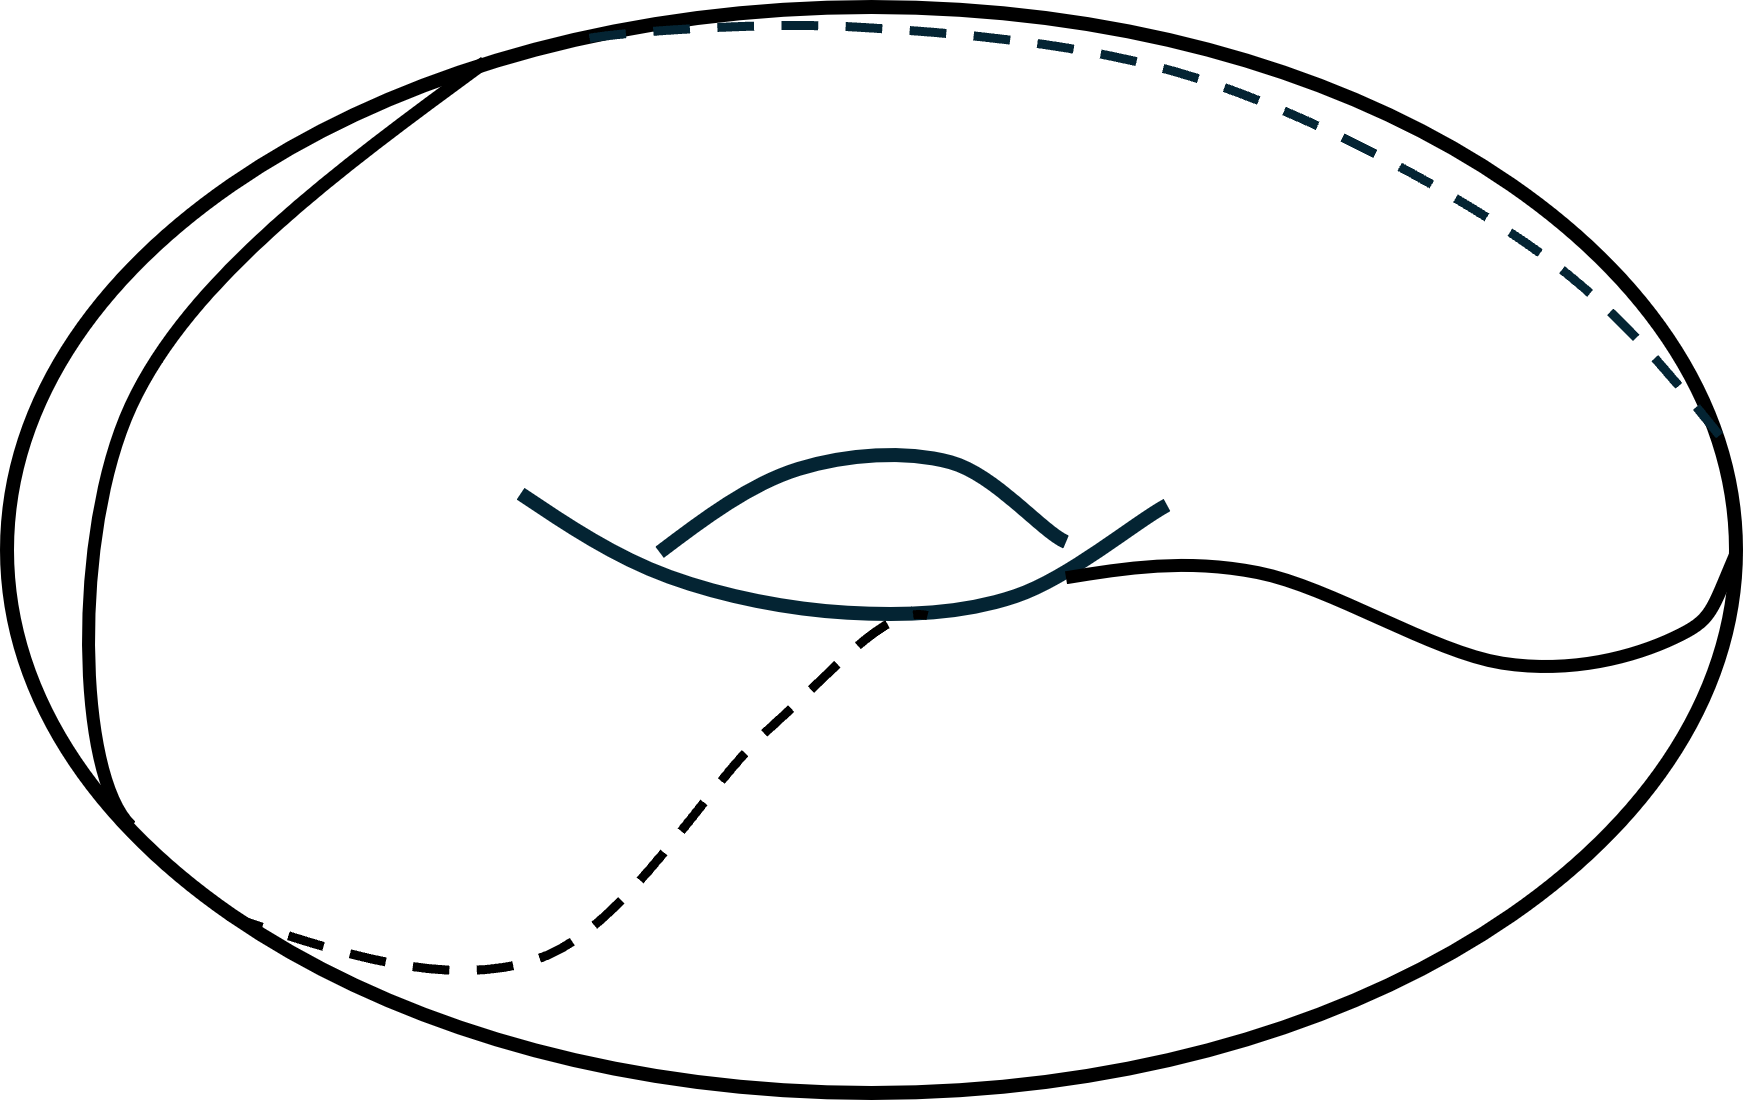
\includegraphics[width=0.25\textwidth]{torusc.png}
\caption{A $(p,q)$ cycle on the torus that carries the twelve-dimensional reduction. A (p,q) 7-brane can be understood as the compactification of the 12d Kaluza-Klein monopole on $T^2$ whose Taub-NUT circle is wrapped on such a (p,q) cycle.
Here being displayed is a (1,1) cycle.}
\label{fig:pq-cycle}
\end{figure}
We now examine the $S,T$ generators of type IIB \SLZ{}.
The $T$ gauge transformation given in \eqref{T gauge transformation} is precisely the type IIB \SLZ{}-$T$ transformation on $\tau$, and the type IIB \SLZ{}-$S$ transformation is achieved with a 12d coordinate swap
\begin{equation}
w_3\to z_1, \quad
z_1\to -w_3 .
\end{equation}
We can thus interpret the type IIB \SLZ{} duality transformations as large gauge transformations in 12d, so that the discrete S and T dualities, ordinarily postulated in 10d, arise geometrically in this 12d picture.

\subsection{D(-1) and D0 interpreted as 12d and 11d pp-waves}
The other $\frac{1}{2}$-BPS solution of the axio-dilaton action \eqref{IIB axio-dilaton action} is the D(-1) instanton, which has been recognised as a 12d pp-wave \cite{Tseytlin:1996ne}.
We now discuss this in the context of the known relation between the D0 brane and an 11d pp-wave.

Pp-waves are solutions of the vacuum Einstein equations following from the Einstein-Hilbert action, describing a gravitational wave propagating at the speed of light.
In $d$ dimensions, written in light-cone coordinates $v,u = z\pm t$, they take the form
\begin{equation}
ds^2 = dudv+(H-1)du^2+\sum_{i=1}^{d-2}dx_i^2,\quad
\nabla^2_{d-2} H(\vec{x})=0,
\label{d-dim pp-wave}
\end{equation}
where the wave profile $H$ is a harmonic function of the $d-2$ transverse coordinates $\vec x$, and the geometry is asymptotically flat as $H\to1$.
For a point source in the transverse space it is standard to take
\begin{equation}
H=1+\frac{Q}{r^{d-4}},
\end{equation}
with $r=|\vec x|$ the transverse radial coordinate.
The constant $Q$ sets the strength of the wave: it is the amplitude of the only metric component deviating from flat space, $g_{uu}=H-1=Q/r^{d-4}$, so $Q\to0$ recovers Minkowski space.
For our purposes, it is in fact more convenient to write \eqref{d-dim pp-wave} instead with explicit $t, z$ coordinates, as
\begin{equation}
ds^2 = - H^{-1}dt^2 + H[dz + (H^{-1} -1)dt]^2 + \sum_{i=1}^{d-2} dx_i^2.
\label{d-dim pp-wave-t-z}
\end{equation}

\paragraph{D0 brane from reduction of the 11d pp-wave}
By specialising \eqref{d-dim pp-wave-t-z} to 11d, we have the 11d pp-wave solution
\begin{equation}
ds_{11}^2
=
-H^{-1}dt^2+H[dz+(H^{-1}-1)dt]^2
+\sum_{i=1}^9 dx_i^2,\quad
H=1+\frac{Q}{r^7}.
\end{equation}
This can be reduced to 10d by comparison with the KK reduction ansatz \eqref{string frame KK reduction ansatz}.
Doing so we find precisely the 10d D0 brane solution in string frame \cite{Stelle:1998xg}
\begin{equation}
ds_{10,string}^2
=-H^{-1/2} dt^2+H^{1/2}ds_9^2,\quad
e^{\Phi} = H^{3/4},\quad
(C_1)_0 = H^{-1}-1.
\end{equation}
Like the relation between the 11d KK-monopole and 10d D6 brane in the type IIA theory, the connection between the 11d pp-wave and the D0 brane is part of the established S-duality between the type IIA theory and M-theory. Despite the absence of a 12d supergravity theory, this story also has a similar analogue on the type IIB side, between a 12d pp-wave and the type IIB D(-1) solution.


\paragraph{D(-1) instanton from reduction of the 12d pp-wave}
We now discuss the parallel story on the type IIB side, specializing \eqref{d-dim pp-wave-t-z} to 12d we find
\begin{equation}
ds_{12}^2 = - H^{-1}dt^2 + H[dz_1 + (H^{-1}-1)dt]^2 + \sum_{i=1}^{10} dx_i^2.
\end{equation}
Performing a Wick rotation via $t = iz_2$ yields
\begin{equation}
ds_{12}^2
= \sum_{i=1}^{10} dx_1^2 + H^{-1}dz_2^2 + H[dz_1 + i(H^{-1}-1)dz_2]^2,
\end{equation}
which, in coordinates $(x^m, z_1, z_2)$, corresponds to the 12d metric embedding
\begin{equation}
\widehat{g}_{MN} = 
\begin{pmatrix}
\delta_{mn} & 0 \\
0 & \hat{g}_{ab}
\end{pmatrix},\quad
\hat{g}_{ab} =
e^{\Phi}\begin{pmatrix}
1 & C_0 \\
C_0 & C_0^2 + e^{-2\Phi}
\end{pmatrix},
\end{equation}
where
\begin{equation}
e^\Phi = H, \quad
C_0 = i (H^{-1}-1).
\end{equation}
This precisely reduces to the D(-1) solution of the type IIB axio-dilaton sector.
Here the axion $C_0$ is purely imaginary, which is a consequence of the Wick rotation we performed to keep the metric real.
It is also customary to define a real scalar $\mathcal C \equiv -i C_0$, which is the axion entering the Euclidean type IIB theory with a wrong sign kinetic term \cite{Gibbons:1995vg}.

% The D(-1) is a solution to the Euclidean type IIB theory, within the axio-dilaton sector \cite{Gibbons:1995vg}.
% In Einstein frame, it can be written as\footnote{In the Euclidean type IIB theory, the compact scalar $C_0$ gets a wrong sign kinetic term, thus becomes purely imaginary. One instead works with $\mathcal C$. This is discussed in \cite{Gibbons:1995vg}.}
% \begin{equation}
% ds_{10}^2 = \sum_{i=1}^{10} dx_i^2,\quad
% e^\Phi = H, \quad
% \mathcal C\equiv-iC_0 = H^{-1}-1,\quad
% H=1+\frac{Q}{r^8}.
% \label{D-1 background}
% \end{equation}
% We now perform its uplift to 12d, using the same ansatz we previously used for relating the D7 brane to the 12d KK-monopole \eqref{12d metric ansatz 0}.
% We find
% \begin{equation}
% ds_{12}^2=
% e^{-\Phi}d\tilde{t}^2+e^\Phi(dy+i\mathcal C d\tilde{t})^2
% +
%  \sum_{i=1}^{10} dx_i^2
% \label{F-theory ansatz}
% \end{equation}
% with $\tilde{t},y$ the coordinates on the torus.
% To keep the metric real, it is natural to perform a Wick rotation $\tilde{t}=-it$, which turns the torus into a non-compact one, and the metric becomes
% \begin{equation}
% ds_{12}^2=
% -e^{-\Phi}dt^2+e^\Phi[dy+\mathcal C dt]^2
% +\sum_{i=1}^{10}dx_i^2.
% \end{equation}
% We thus find the 12d metric
% \begin{equation}
% ds_{12}^2
% =
% dudv
% +(H-1)du^2
% +ds_{10}^2,\quad
% v,u = y\pm t.
% \end{equation}
% By comparison with \eqref{d-dim pp-wave}, we see that the uplift of D(-1) is a pp-wave in 11+1 dimensions.
One may view the Euclidean D(-1) as a ``slice'' of the 10d homogeneous wavefront of a 12d pp-wave.
The momentum of the wave is the D(-1) charge.
Recent investigations of the IKKT matrix model \cite{Hartnoll:2024csr,Komatsu:2024bop} reveal a type IIB supergravity background with axio-dilaton and the 3-form turned on, which admits a similar 12d interpretation.\footnote{
The mass-deformed model is dual to a probe D1 brane in the Einstein-frame-flat background $ds_{10}^2 = \sum_i dx_i^2$, $e^\Phi = 1 - \frac{\mu^2}{32}\left(\sum_{A=1}^7 x_A^2 + 3\sum_{a=9}^{10}x_a^2\right)$, $H_3 = \mu dx^8\wedge dx^9\wedge dx^{10}$, valid in the ellipsoidal region where $e^\Phi\ge0$ \cite{Hartnoll:2024csr}. Uplifting to 12d (Wick rotating to keep $ds^2$ real) gives the Brinkmann-form metric $ds_{12}^2 = 2dudv + e^\Phi du^2 + \sum_{i=1}^{10}dx_i^2$, whose only non-vanishing Ricci component is $R_{uu}=\mu^2/2$. Since $e^\Phi$ is not harmonic it is not a pp-wave, but it solves 12d gravity coupled to a 4-form, $S = \int d^{12}x\sqrt{-\widehat{g}}\left(\widehat{R}-\tfrac12|\widehat{F}_4|^2\right)$ with $\widehat{F}_4 = \mu du\wedge dx^8\wedge dx^9\wedge dx^{10} = du\wedge H_3$.
}

\subsection{Supersymmetry}
We now discuss a further consistency check for the relation between 12d gravity and the type IIB axio-dilaton sector, namely how the $\tfrac{1}{2}$ BPS condition of the latter can be obtained by reducing the covariantly-constant equation of the former.

Disregarding the type IIB supergravity action for the moment, let us consider a generic theory in $d$ dimensions.
The action with kinetic terms for the metric, form fields, and the gravitino takes the form
\begin{equation}
S = \int d^d x  \sqrt{-g}\left[
R
- \frac{1}{2}\sum_n \frac{1}{n!} |F_n|^2
- i \bar{\psi}_M \Gamma^{MNP} \nabla_N \psi_P
\right] + \dots.
\label{generic sugra action}
\end{equation}
Under a local supersymmetry transformation parameterised by a spinor $\epsilon$, one can write down a general equation for the variation of the gravitino from covariance alone
\begin{equation}
\delta\psi_M
= \left\{
\nabla_M + \sum_n \left[
c_n (F_{n})_M{}^{N_1 N_2 \cdots} \Gamma_{N_1 N_2 \cdots}
+ d_n (F_{n})_{N_1 N_2 \cdots} \Gamma_M{}^{N_1 N_2 \cdots}
\right]
\right\}\epsilon,
\label{generic gravitino variation}
\end{equation}
with summation over the form fields of the given theory, and $c_n, d_n$ are coefficients to be determined.
The Killing spinor equation would then be given by $\delta\psi_M=0$.

Upon dimensional reduction, the higher-dimensional fields decompose into those of the lower-dimensional theory, and the reduction of the gravitino variation \eqref{generic gravitino variation} reproduces the lower-dimensional Killing spinor equation.
In our case the higher-dimensional theory is pure gravity, with no form fields, so its gravitino variation \eqref{generic gravitino variation} is simply $\nabla_M\epsilon$.
The full lower-dimensional Killing spinor equation, flux and connection terms included, must then be reproduced by reducing this covariant derivative alone.

\paragraph{From 11d to type IIA.}
Let us consider the 11d covariant constancy equation $\widehat{\nabla}_M \epsilon = 0$.
Splitting the 11d indices into $x^M = (x^m, x^{11})$, we have
\begin{equation}
\begin{aligned}
\widehat{\nabla}_m \epsilon 
&= \nabla_m \epsilon + \frac{1}{4} \widehat{w}_{mBC} \Gamma^{BC} \epsilon = 0,\\  
\widehat{\nabla}_{11} \epsilon 
&= \frac{1}{4} \widehat{w}_{11,BC} \Gamma^{BC} \epsilon = 0.
\end{aligned}
\end{equation}
Substituting the reduced spin connection (see \cite{Ortin:2015hya}) on the standard Kaluza-Klein ansatze \eqref{string frame KK reduction ansatz}, they become
\begin{equation}
\begin{aligned}
\widehat{\nabla}_m \epsilon
&= e^{\Phi/3}\left[ \nabla_m - \frac{1}{6} \Gamma_m{}^n \partial_n \Phi + \frac{1}{4} e^\Phi F_{mn} \Gamma^n \Gamma^{11} \right] \epsilon = 0,\\
\widehat{\nabla}_{11} \epsilon
&=\frac{1}{4} e^{Phi/3} \left[ -\frac{1}{2} e^{\Phi} F_{mn} \Gamma^{mn} - \frac{4}{3}\partial_m \Phi \Gamma^m \Gamma^{11} \right] \epsilon = 0.
\end{aligned}
\end{equation}
We can substitute the $\widehat{\nabla}_{11} \epsilon = 0$ equation into the $\widehat{\nabla}_m \epsilon = 0$ equation to find
\begin{equation}
\nabla_m \epsilon = e^{\Phi/3} \left[ \nabla_m + e^\Phi \left(\frac{1}{8}F_{mn}\Gamma^n - \frac{1}{16}F_{nr}\Gamma_m{}^{nr}\right) \Gamma^{11} + \frac{1}{6}\partial_m\Phi \right] \epsilon = 0.
\end{equation}
The flux term can be simplified in the following manner:
\begin{equation}
\begin{aligned}
\frac{1}{8}F_{mn}\Gamma^n - \frac{1}{16}F_{nr}\Gamma_m{}^{nr}
&= -\frac{1}{16}F_{nr}(\Gamma_m{}^{nr} - 2\delta_m^{[n}\Gamma^{r]})\\
&= - \frac{1}{8}F_{nr}\{\Gamma_m,\Gamma^{nr}\}\\
&= - \frac{1}{8} F_{nr} \Gamma_m{}^{nr}.
\end{aligned}
\end{equation}
Then performing a redefinition $\epsilon \to e^{-\Phi/6} \epsilon$ to remove the $\partial\Phi$ term, we arrive at
\begin{equation}
\left(
\nabla_m - \frac{1}{8}e^\Phi F_{nr} \Gamma_m{}^{nr}\Gamma^{11}
\right)\epsilon = 0,
\end{equation}
which is precisely the type IIA Killing spinor equation in the gravity, KK-vector and dilaton sector \cite{Becker:2006dvp}.
Hence the 10d $\tfrac{1}{2}$ BPS condition may be understood from 11d covariance.
Now we present an analogous story between 12d covariance and the type IIB theory.

% Let us consider the equation $\widehat{\nabla}_M \epsilon = 0$ that states the covariant constancy of an 11d spinor $\epsilon$.
% Splitting the 11d indices into 10d spacetime and the M-theory circle, we have
% \begin{equation}
% \begin{aligned}
% \widehat{\nabla}_m \epsilon = \nabla_m \epsilon + \frac{1}{4} \widehat{w}_{mBC} \Gamma^{BC} \epsilon &= 0,\\
% \widehat{w}_{11,BC} \Gamma^{BC} \epsilon &= 0.
% \end{aligned}
% \end{equation}
% Substituting the reduced spin connection (see \cite{Becker:2006dvp}) for the standard Kaluza-Klein ansatz \eqref{string frame KK reduction ansatz}, we find
% \begin{equation}
% \begin{aligned}
% \widehat w_{aBC}\Gamma^{BC}
% &=e^{\Phi/3}\left[w_{abc}\Gamma^{bc}-\tfrac23\Gamma_a{}^b\partial_b\Phi\right]+e^{4\Phi/3}F_{ab}\Gamma^b\Gamma^{11},\\
% \widehat w_{11,BC}\Gamma^{BC}
% &=-\tfrac12 e^{4\Phi/3}F_{bc}\Gamma^{bc}-\tfrac43 e^{\Phi/3}\partial_m\Phi\Gamma^m\Gamma^{11}.
% \end{aligned}
% \end{equation}
% Hence the 11d covariant constancy condition reduces to
% \begin{equation}
% \begin{aligned}
% \left[-\tfrac12 e^\Phi F_{bc}\Gamma^{bc}-\tfrac43\partial_m\Phi\Gamma^m\Gamma^{11}\right]\epsilon &= 0\\
% \left[\nabla_m-\tfrac16\Gamma_m{}^n\partial_n\Phi+\tfrac14 e^\Phi F_{mn}\Gamma^n\Gamma^{11}\right]\epsilon &= 0.
% \label{IIA spacetime gravitino}
% \end{aligned}
% \end{equation}
% The first equation is algebraic in $\epsilon$. Multiplying by $\Gamma^{11}$ and using $(\Gamma^{11})^2=1$, it becomes the type IIA dilatino variation
% \begin{equation}
% \Gamma^b\partial_b\Phi\epsilon=\tfrac38 e^\Phi F_{bc}\Gamma^{bc}\Gamma^{11}\epsilon .
% \label{IIA dilatino relation}
% \end{equation}
% We now use \eqref{IIA dilatino relation} to remove $\partial\Phi$ from the spacetime equation \eqref{IIA spacetime gravitino}.
% Writing $\Gamma_m{}^n\partial_n\Phi=\Gamma_m(\Gamma^n\partial_n\Phi)-\partial_m\Phi$ and inserting \eqref{IIA dilatino relation}, the flux term it produces combines with the $\tfrac14 e^\Phi F_{mn}\Gamma^n\Gamma^{11}$ already present, giving
% \begin{equation}
% \widehat\nabla_m\epsilon=e^{\Phi/3}\left(\nabla_m+\tfrac16\partial_m\Phi+\tfrac18 e^\Phi F_{mn}\Gamma^n\Gamma^{11}-\tfrac1{16}e^\Phi F_{np}\Gamma_m{}^{np}\Gamma^{11}\right)\epsilon ,
% \label{IIA assembled}
% \end{equation}
% where we used $\Gamma_m\Gamma^{np}=\Gamma_m{}^{np}+2\delta_m^{[n}\Gamma^{p]}$.
% The rank-one and rank-three flux terms then recombine into a single flux-slash acting on $\Gamma_m$: with $\Gamma^{np}\Gamma_m=\Gamma_m{}^{np}-2\delta_m^{[n}\Gamma^{p]}$,
% \begin{equation}
% \tfrac18 F_{mn}\Gamma^n-\tfrac1{16}F_{np}\Gamma_m{}^{np}=-\tfrac1{16}F_{np}\Gamma^{np}\Gamma_m .
% \end{equation}
% Finally, the Weyl rescaling $\epsilon\to e^{-\Phi/6}\epsilon$ removes the $\tfrac16\partial_m\Phi$ term, leaving us precisely with the type IIA Killing spinor equation in the gravity, KK-vector and dilaton sector,
% \begin{equation}
% \delta \psi_m =
% \left(
% \nabla_m - \tfrac{1}{16}e^\Phi F_{np}\Gamma^{np}\Gamma_m\Gamma^{11}
% \right)\epsilon = 0.
% \label{IIA Killing spinor equation}
% \end{equation}

\paragraph{From 12d to type IIB.}
A 12d covariant derivative $\widehat{\nabla}^{(12)}_M\epsilon = 0$ restricted to 10d coordinates $x^m$ takes the form
\begin{equation}
\nabla^{(12)}_m\epsilon
=\left(
\nabla^{(10)}_m
+\frac{1}{2}\widehat{w}_m{}^{11,n}\Gamma_{11,n}
+\frac{1}{2}\widehat{w}_m{}^{12,n}\Gamma_{12,n}
+\frac{1}{2}\widehat{w}_m{}^{11,12}\Gamma_{11,12}\right)\epsilon = 0,
\label{12d covariant derivative}
\end{equation}
Using the 12d metric ansatz, we find the spin connections
\begin{equation}
\widehat{w}_m{}^{11,n}=\widehat{w}_m{}^{12,n}=0,\quad
\widehat{w}_m{}^{11,12} = -\frac{1}{2}\frac{\partial_m \tau_1}{\tau_2}.
\end{equation}
The 12d covariant derivative \eqref{12d covariant derivative} thus becomes
\begin{equation}
\left[
\nabla_m + \frac{1}{2} Q_m \Gamma_{11,12}
\right]\epsilon,
\end{equation}
where $Q_m = -\frac{1}{2} \frac{\partial_m \tau_1}{\tau_2}$ is the non-dynamical U(1) connection the type IIB axio-dilaton sector.
We note that on a Euclidean torus
\begin{equation}
\Gamma_{11,12} = \Gamma_{11}\Gamma_{12},\quad
(\Gamma_{11,12})^2 =-\Gamma_{11}^2\Gamma_{12}^2 = -1,
\end{equation}
so $\Gamma_{11,12}$ is, up to a similarity transformation, $i$ times the U(1) generator.
After performing a similarity transformation one obtains precisely the axio-dilaton sector Killing spinor equation \eqref{9+1 IIB axio-dilaton Killing spinor equations}.
This would also hold had we compactified a non-compact torus instead, to obtain a Euclidean type IIB theory.
In the case of compactifying on a torus of signature (1,1), a factor of $i$ arises both in identifying the U(1) generator from $\Gamma_{11,12}$ and in defining the Euclidean compact scalar $C_0 = i\mathcal C$, so that the 12d covariant derivative again reproduces the type IIB gravitino variation.
